\chapter{Semantics-First Approach to Clinical Decision Support}

In \autoref{chapter:introduction}, we explained that, despite
advances in medicine, mortality and costs associated with preventable
medical errors (\PMEs{}) remain unacceptably high. In
\autoref{chapter:background}, we explained how systems that
assist healthcare practitioners (\HCPs{}) with situation-specific
advice based on evidence-based best practice guidelines (\BPGs{}),
called clinical decision (\CDSSs{}) can reduce both mortality
and costs associated with \PMEs{}. But, despite their potential,
the uptake of such systems in practice is hindered by challenges
that were introduced in \autoref{sec:hurdles-cdss-adoption}, and
discussed in depth in \autoref{chapter:hurdles-cdss-adoption}.
In brief, the following challenges (Cs) were outlined:
\begin{enumerate}[label=C\arabic*.]
\itemsep0.0em
\item Absence of systematic ways of \emph{validating content}
in a \emph{reliable}, \emph{accessible} and \emph{updateable} manner.
\item Lack of \emph{reliable}, \emph{shareable} \CDSS{} content
that can be easily adopted across healthcare organizations and their (Information
Technology) \IT{} systems.
\item Technical difficulties of sharing due to \emph{need for
  adaptation} to diverse Electronic Health Records (\EHR) systems.
\item \emph{Suboptimal} User Interfaces (\UIs), implementation choices and
workflows.
\end{enumerate}

\begin{figure}[th!]
  \centering
  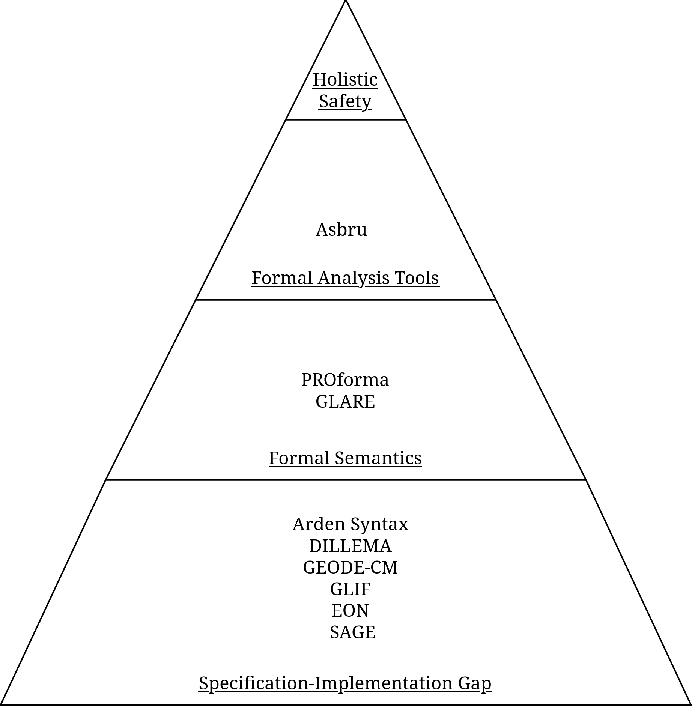
\includegraphics[width=0.5\textwidth]{pyramid}
  \caption{Existing \DSLs{} for Computer Interpretable Guidelines}\label{fig:existing-work-pyramid}
\end{figure}

Over the years, significant progress has been made towards
addressing these challenges. In \autoref{chapter:related-work},
we discussed how existing approaches have attempted to
address said challenges, and their limitations. Specifically,
in \autoref{sec:related-work-discussion}, we outlined major
themes that these approaches adopt to tackle these challenges.
This is further illustrated by the pyramid diagram in \autoref{fig:existing-work-pyramid}, where aforementioned themes are
underlined in the pyramid's various rungs.
As is typical, approaches that appear in higher rungs also
have characteristics of ones below them. For example, while guidelines expressed in
the Arden Syntax eliminate the specification-implementation gap by being
both \HCP{}-comprehensible and interpretable, they cannot be formally analyzed
due to lack of analysis tools in the ecosystem. Asbru-based guidelines
on the other hand not only eliminate the specification-implementation gap, but can also be
formally analyzed using support for KIV-based verification in the Asbru
ecosystem (see \autoref{sec:kiv-verification}).

As is evident in \autoref{fig:existing-work-pyramid}, no
existing approach covers the \say{holistic safety} rung of the pyramid.
Recall from \autoref{sec:related-work-discussion} that we say an
approach tackles \say{holistic safety} if,
besides support for analyzing guidelines,
analysis and execution tools also have correctness guarantees.
In this work, we argue that such guarantees are necessary for
trustworthy \CDSSs{}. We attempt to address \say{holistic safety}
systematically by developing a \emph{semantics-first approach} for
building clinical decision support systems. In this context, by semantics-first
we mean that:
\begin{itemize}
  \item The semantics of the programming language for defining said knowledge is
    formally defined, from which execution and analysis tools are derived in a
    correct by construction manner, leading to holistic safety.
  \item The semantics of medical knowledge are expressed accurately.
\end{itemize}
At the core of our approach is a novel domain-specific language for expressing
medical knowledge called $\MediK{}$ (pronounced Medi-Kay). By being comprehensible to domain experts
in medicine, $\MediK{}$-based computer interpretable guidelines can serve
both as a guideline's non-executable \HCP{}-comprehensible description, i.e.,
the specification, and its encoding in a computable medium, i.e., the
implementation, thereby eliminating any specification-implementation gap.

The remainder of this chapter is structured as follows:
\autoref{sec:semantics-first} briefly describes the semantics-first philosophy.
Next, \autoref{sec:k-framework} describes $\K$ -- the language semantic
framework that $\MediK{}$'s are expressed in. Finally,
\autoref{sec:semantics-first-pitfalls} describes potential pitfalls
of following the semantics-first philosophy.

\section{Semantics-First Approach}\label{sec:semantics-first}

The semantics-first approach prescribes a systematic way of
developing programming languages. Instead of implementing
tools for a language, such as interpreters, compilers and
model checkers in ad-hoc manner, the approach states that the
first step in developing said tools must be to formally define
the language's semantics. As show in \autoref{fig:semantics-first},
once defined, all tools for the language
can then be automatically derived from the semantics. Moreover, since
the tools utilize the semantics, they are, by definition,
correct-by-construction.

While following the semantics-first philosophy might seem like an obvious choice
in language design, its adoption in practice is far from ideal.
Conventional practice in the programming language and formal
methods community is still to develop analysis and execution tools for each
programming language from scratch \cite{ChenSETSS19}, as illustrated
in \autoref{fig:conventional-pl-development} from
\cite{ChenSETSS19}. But, this approach has several
disadvantages:
\begin{itemize}
  \item Implementing tools that perform the same function for
    different languages incurs unnecessary development and maintenance cost.
    As shown in \autoref{fig:conventional-pl-development}, if there are
    $l$ languages, where each has $t$ tools, then a total of $l \times t$
    tools have to be developed and maintained over time.
  \item Tools are often based on informal descriptions of language semantics,
    leaving developers to extrapolate finer details of the language's semantics,
    leading to inconsistencies.
    For instance, in \cite{ParkPLDI15}, it was found
    that ECMAScript 5.1-compliant JavaScript engines
    in mainstream web browsers behaved differently from each other
    for certain complex JavaScript programs.
  \item As newer versions of a language are introduced, each
    tool for the language has to be updated to ensure support for the latest
    version. This again results in duplicated work.
\end{itemize}
\begin{figure}[t!]
  \centering
  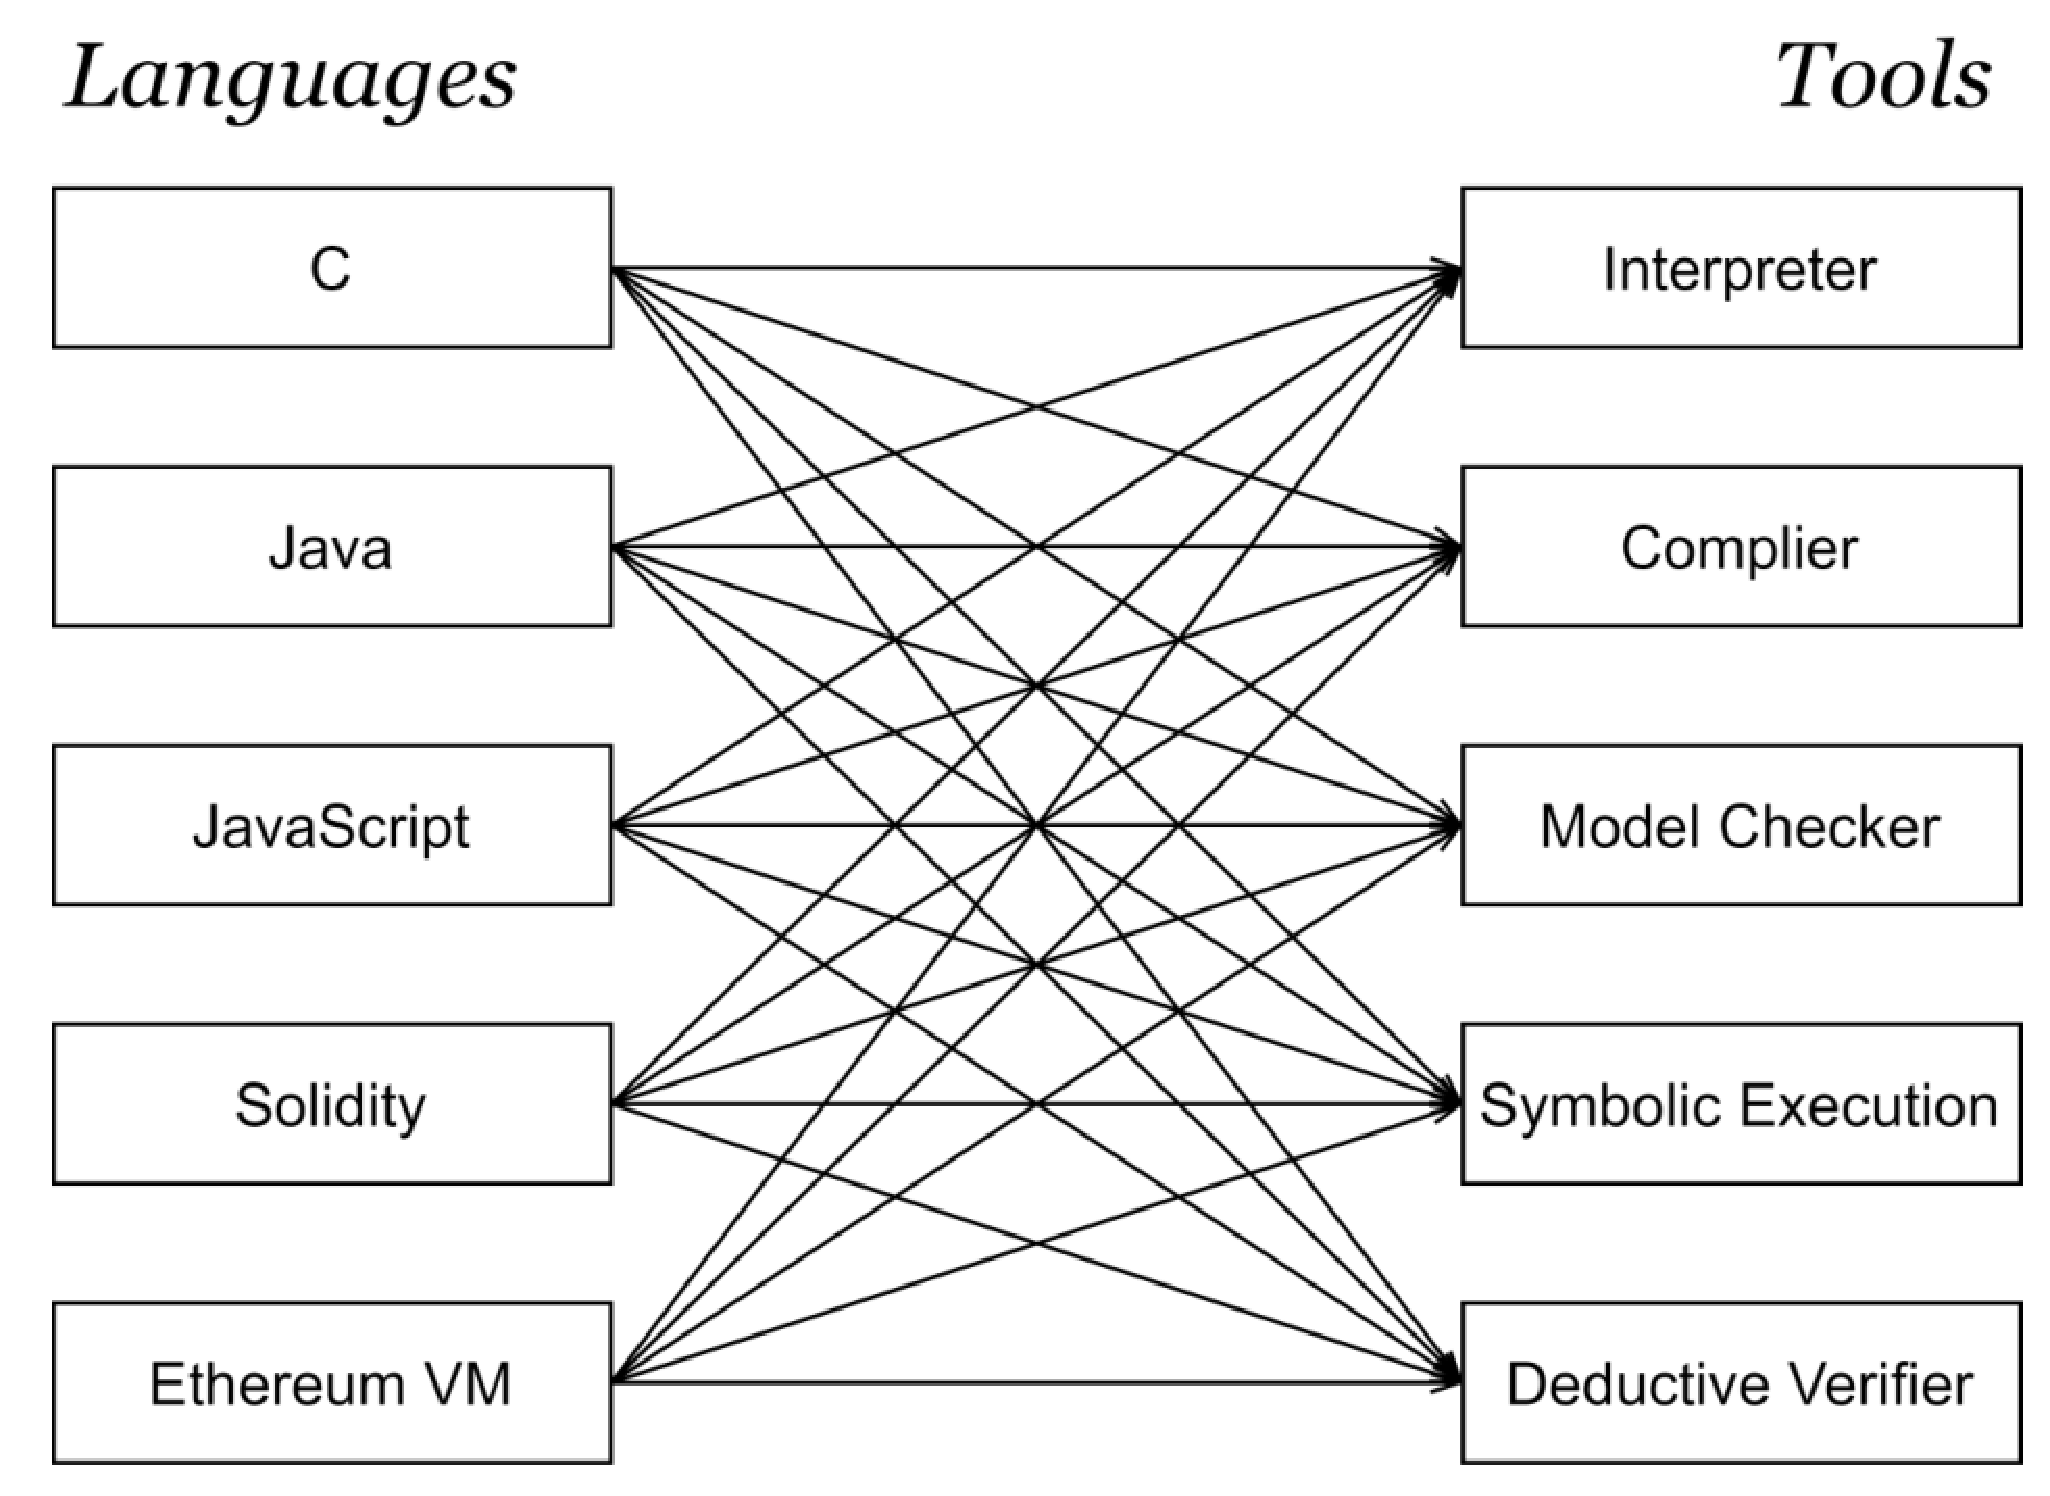
\includegraphics[width=0.6\textwidth]{conventional-pl-development}
  \caption{State-of-Art in Programming Language Design}\label{fig:conventional-pl-development}
\end{figure}

\subsection{Why build \CDSSs{} using Semantics-First?}

In section \ref{sec:semantics-first}, we described benefits
of using the semantics-first approach for developing regular programming
language. But, these differences become starker when semantics-first
is compared against the conventional approach shown in \autoref{fig:conventional-pl-development} in context of domain-specific language for
expressing medical guidelines. Specifically, as such a language will be utilized
in safety-critical settings, it is vital that the language:
\begin{itemize}
  \item Has an \emph{unambiguous}, \emph{formal}
    semantics that can serve as a reference for developing tool support for it.
    This is necessary to ensure that
    tools are free of behavioral inconsistencies due to ambiguities in the
    semantics.
  \item Is supported by a rich formal analysis tools that can
    be used to analyze programs.
    Implementing such tools from scratch would require significant effort.
  \item Can evolve quick to incorporate
    \begin{enumerate*}[label=(\roman*)]
      \item lessons from expressing medical guidelines in it, and,
      \item \HCP{} feedback, specifically regarding comprehensibility.
    \end{enumerate*}
    This can be challenging when using the approach shown in \autoref{fig:conventional-pl-development}, as
    every change to the language's semantics would require corresponding
    changes to all relevant tools, and additional effort to maintain
    different versions, making the development process extremely tedious.
\end{itemize}

\section{The $\K{}$ Framework}\label{sec:k-framework}

In this section, we introduce $\K{}$: a rewrite-based executable semantics
in which programming languages can be defined through configurations and rules
\cite{KframeworkUrl}. Once the semantics of a programming language has been
defined, $\K{}$ automatically generates all tools depicted in \autoref{fig:semantics-first}, such as an interpreter, compiler,
model-checker and deductive verifier for the language. $\K{}$ has been successfully
utilized to formalize semantics of large real-world languages, such as
C \cite{HathhornPLDI15}, Java \cite{BogdanasPOPL15} and
Javascript \cite{ParkPLDI15}, and analyze non-trivial programs
\cite{StefanescuOOPSLA16,ParkFSE18}.

The remainder of this section introduces relevant features of
$\K{}$ by describing the $\K{}$ semantics of an example language called
Imp. This introduction to $\K{}$ provides necessary background
for upcoming chapters that discuss the $\MediK{}$ \DSL{} through the
use of $\K{}$ notation and concepts.

\subsection{Defining Languages in $\K$}\label{sec:semantics-in-k}

A typical $\K$ definition of a language consists of the following components:
\begin{itemize}
  \item Syntax: Defined in \BNF{}-like notation, and utilized by $\K$
    to generate a parser for the language.
  \item Configuration: Organizes the program execution state
    into units called \emph{cells} that may be nested.
  \item Rules: Operate over configuration segments and define program
    evolution via rewrites.
\end{itemize}
We now discuss aforementioned components in the context of the Imp
language. Imp is a simple imperative programming language
inspired by C and Java that supports arithmetic and boolean expressions and
statements such as variable declaration and assignment, branching (\inlinek{if})
and looping (\inlinek{while}).

\autoref{lst:imp-syntax} and \autoref{lst:imp-semantics},
define syntax and semantics of Imp respectively.
$\K{}$ code must be place inside an organizational unit called a
\inlinek{module} that has a name, and can import other \inlinek{module}(s).
For example, \inlinek{module IMP-SYNTAX ... endmodule}
between \autoref{lstline:imp-module-start} and
\autoref{lstline:imp-module-end} of \autoref{lst:imp-syntax} defines
a $\K{}$ \inlinek{module} named \inlinek{IMP-SYNTAX} containing Imp's
grammar. $\K{}$ provides builtin support for domains such as natural
numbers, integers, booleans and program identifiers
under a \inlinek{module} named \inlinek{DOMAINS}.
\autoref{lstline:imp-syntax-import} \inlinek{imports}
the syntax definition of $\K{}$'s \inlinek{DOMAINS} module
to enable parsing integers and booleans in Imp programs.

\begin{lstlisting}[float=ht,
  frame=single,
  style=ksty,
  language=k,
  numbers=left,
  numbersep=5pt,
  caption={Imp Syntax in $\K$},
  label={lst:imp-syntax},
  xleftmargin=3ex
]
module IMP-SYNTAX                                               @\label{lstline:imp-module-start}@
  imports DOMAINS-SYNTAX                                        @\label{lstline:imp-syntax-import}@
  syntax AExp  ::= Int | Id                                     @\label{lstline:imp-aexp-start}@
                 | "-" Int
                 | AExp "/" AExp              [left, strict]    @\label{lstline:imp-aexp-div}@
                 | "(" AExp ")"               [bracket]
                 > AExp "+" AExp              [left, strict]    @\label{lstline:imp-aexp-end}@
  syntax BExp  ::= Bool
                 | AExp "<=" AExp             [seqstrict]
                 | "!" BExp                   [strict]
                 | "(" BExp ")"               [bracket]
                 > BExp "&&" BExp             [left, strict(1)] @\label{lstline:imp-bexp-and}@
  syntax Block ::= "{" "}"
                 | "{" Stmt "}"
  syntax Stmt  ::= Block                                        @\label{lstline:imp-stmt-block}@
                 | Id "=" AExp ";"            [strict(2)]       @\label{lstline:imp-stmt-assgn}@
                 | "if" "(" BExp ")"
                   Block "else" Block         [strict(1)]
                 | "while" "(" BExp ")" Block                   @\label{lstline:imp-stmt-while}@
                 > Stmt Stmt                  [left]            @\label{lstline:imp-stmt-comp}@
  syntax Pgm ::= "int" Ids ";" Stmt                             @\label{lstline:imp-pgm}@
  syntax Ids ::= List{Id,","}                                   @\label{lstline:imp-ids}@
endmodule                                                       @\label{lstline:imp-module-end}@
\end{lstlisting}

\emph{Syntax} in $\K{}$ is defined using BNF-like notation; terminals are enclosed
in quotes, and non-terminals begin with an uppercase. For example,
consider the declaration of Imp arithmetic expressions between
\autoref{lstline:imp-aexp-start} and \autoref{lstline:imp-aexp-end}. On
\autoref{lstline:imp-aexp-start} $\K$'s builtin support
for integers (\inlinek{Int}) and program identifiers
(\inlinek{Id}) is used to support arithmetic expressions over program variables.
Beyond simply defining the syntax, $\K{}$ also allows assigning semantics to
constructs through the use of \emph{attributes} specified as a comma-separated list
inside square brackets (\inlinek{[..]}) placed immediately after the \BNF{} production.
For example, On \autoref{lstline:imp-aexp-div} and \autoref{lstline:imp-aexp-end},
the attribute \inlinek{left} is used to declare the
corresponding operator as left associative. The \inlinek{strict} attribute is used
to assign \emph{evaluation strategies}. Note its use
on \autoref{lstline:imp-aexp-div} and \autoref{lstline:imp-aexp-end}, signifying
that both operand sub-expressions must be completely evaluated before the
before the corresponding operator (\inlinek{/}, \inlinek{+}) is evaluated.
Note that the order in which the arguments are evaluated is non-deterministic,
and, all operands will be evaluated before the operator is evaluated.
To enforce a particular order, or, to choose a subset of the operands, a
list of operand positions specifying the desired order can be supplied to
\inlinek{strict}. For example, \inlinek{strict(2, 1)} would make $\K$
evaluate the second argument before the first. This is particularly
useful for defining constructs like short-curcuit (\inlineimp{&&}) boolean
expression on \autoref{lstline:imp-bexp-and}, where \inlinek{strict(1)}
ensures that the left operand is evaluated first, allowing the right to only
be evaluated if the left evaluates to \inlinek{true}.
Similarly, for an assignment statement on \autoref{lstline:imp-stmt-assgn}
the \inlinek{strict(2)} indicates that the second argument, i.e., the
expression to the right of the \inlineimp{=} sign must be evaluated before
the identifier on the left of the \inlineimp{=} is updated.

$\K{}$ also allows operator precedence to be specified as a part of the
syntax definition. On \autoref{lstline:imp-aexp-end},
the \inlinek{>} signifies that all preceding productions have higher precedence,
i.e., bind tighter, than the production for addition (\inlinek{+}).
Similarly, \autoref{lstline:imp-stmt-comp} defines statement composition.
Thus, preceding \inlinek{Stmt} productions
(\autoref{lstline:imp-stmt-block}-\autoref{lstline:imp-stmt-while}), that define
blocks (\inlinek{\{..\}}) and standalone statements such as variable assignment and
while loop have higher precedence, indicated by \inlinek{>} on \autoref{lstline:imp-stmt-comp}.

On \autoref{lstline:imp-pgm}, an Imp program is defined to start with a list of program variable
declarations (\inlinek{"int" Ids ";"}) followed by other statements. Note the
definition of a list of identifier (\inlinek{Ids}) on \autoref{lstline:imp-ids}. In $\K{}$,
\inlinek{List\{...\}} is used to define syntactic-lists, where the first
argument is the production of list elements, and the second the list de-limiter.
Thus, \inlinek{List\{Id, ","\}} defines a comma-separated list of program identifiers.

Once the \emph{syntax} has been defined, $\K$ can utilize it to generate a
parser, which can be used to generate abstract
syntax trees (\ASTs{}) for programs. The program's \AST{} forms a part of the larger
program state, over which semantics are defined through rules.
The $\K$ semantics of any language has two components:
\begin{itemize}
  \item A \emph{Configuration} that organizes the state
    into units called \emph{cells}, that may be nested.
  \item \emph{Rules} that operate over \emph{configuration}-segments
    to desribe evolution of state during execution.
\end{itemize}
For Imp, \autoref{lst:imp-semantics} has aforementioned
components inside \inlinek{module IMP}.
Note that the syntax and semantics exist in separate modules,
where the semantics module \inlinek{imports}
the syntax module. This is by convention, and
has the following advantages:
\begin{enumerate}[label=\alph*)]
  \item Rules can operate directly over the language's syntax,
    making them easier to specify and comprehend.
  \item With the syntax and semantics residing in separate modules,
    $\K$ can be instructed to use only the syntax module for parsing programs.
    This allows users to define additional syntactic constructs in the semantics module
    for use in rules. If a combined syntax and semantics module is used instead,
    any constructs defined solely for use in rules
    would unintentionally become part of the language's syntax,
    and be accepted by the parser.
\end{enumerate}

\begin{lstlisting}[float=t,
  frame=single,
  style=ksty,
  language=k,
  numbers=left,
  numbersep=5pt,
  caption={$\K$ Semantics of Imp},
  label={lst:imp-semantics},
  xleftmargin=3ex
]
module IMP
  imports IMP-SYNTAX
  imports DOMAINS
  syntax KResult ::= Int | Bool             @\label{lstline:imp-kresult}@

  configuration <T>                         @\label{lstline:imp-config-start}@
                  <k> $PGM:Pgm </k>         @\label{lstline:imp-pgm-var}@
                  <state> .Map </state>     @\label{lstline:imp-pgm-state}@
                </T>                        @\label{lstline:imp-config-end}@

// AExp
  rule <k> X:Id => I ...</k> <state>... X |-> I ...</state> @\label{lstline:imp-lookup-rule}@
  rule I1 / I2 => I1 /Int I2  requires I2 =/=Int 0
  rule I1 + I2 => I1 +Int I2                @\label{lstline:imp-add-rule}@
  rule - I1 => 0 -Int I1
// BExp
  rule I1 <= I2 => I1 <=Int I2
  rule ! T => notBool T
  rule true && B => B @\label{lstline:imp-and-true-rule}@
  rule false && _ => false @\label{lstline:imp-and-false-rule}@
// Block
  rule {} => .   [structural]
  rule {S} => S  [structural]
// Stmt
  rule <k> X = I:Int; => . ...</k> <state>... X |-> (_ => I) ...</state> @\label{lstline:imp-assgn-rule}@
  rule S1:Stmt S2:Stmt => S1 ~> S2  [structural] @\label{lstline:imp-stmt-decomp-rule}@
  rule if (true)  S else _ => S  @\label{lstline:imp-if-true-rule}@
  rule if (false) _ else S => S  @\label{lstline:imp-if-false-rule}@
  rule while (B) S => if (B) {S while (B) S} else {}  [structural]
// Pgm
  rule <k> int (X,Xs => Xs);_ </k> <state> Rho:Map (.Map => X|->0) </state> @\label{lstline:imp-vardec-rule}@
    requires notBool (X in keys(Rho))  @\label{lstline:imp-vardec-requires}@
  rule int .Ids; S => S  [structural]  @\label{lstline:imp-emptydec-rule}@

endmodule
\end{lstlisting}

\subsubsection{Configurations}\label{sec:k-configuration}

The configuration is defined using the keyword \inlinek{configuration},
followed by an unordered list of \emph{cells},
which may be nested and are specified using an XML-like notation.
For instance, \inlinek{<foo> <bar> ... </bar> </foo>}
corresponds to $\K$ \emph{cells} named
\inlinek{foo} and \inlinek{bar} respectively, where \inlinek{bar}
is nested under \inlinek{foo}.
Imp's configuration is defined
between \autoref{lstline:imp-config-start} and \autoref{lstline:imp-config-end},
and consists of a top-level cell \inlinek{<T>} containing cells
\inlinek{<k>} and \inlinek{<state>} on \autoref{lstline:imp-pgm-var} and
\autoref{lstline:imp-config-end} respectively. In $\K{}$,
the \inlinek{<k>} cell typically contains the \AST{} of the executing
program, indicated by its contents \inlinek{$PGM:Pgm}.
During execution, $\K{}$ will attempt to parse the program being executed
using the production \inlinek{Pgm} defined on \autoref{lstline:imp-pgm} of
\autoref{lst:imp-syntax}. If parsing is successful, $\K{}$ will replace
\inlinek{$PGM} with the parsed \AST{}. The \inlinek{<state>} cell,
as the name suggests, will hold a map of
program identifiers and values they acquire during execution.
Said map is initially empty, denoted by \inlinek{.Map}.
The dot (\inlinek{.}) in $\K{}$ denotes \emph{nothing} or \emph{empty}.
Thus, \inlinek{.Map} denotes an empty map.

\subsubsection{Rules}\label{sec:k-rules}
$\K$ \emph{rules} operate over configuration segments and define evolution of
program state. When specifying a rule $\K{}$, only relevant parts of the
configuration need to be mentioned---$\K{}$ completes the rest of the
configuration through a mechanism called \emph{configuration abstraction}.
This allows rules to be concise,
enhancing readability and making them easier to write. For example,
consider the rule for addition on \autoref{lstline:imp-add-rule}.
Simply put, the rule specifies that if the term at the top of the \inlinek{<k>}
cell is an addition expression, then it should be \emph{rewritten} to
addition in the integer domain \inlinek{+Int}. But, even though the
rule is intended to simplify the top of the \inlinek{<k>} cell,
no cells are explicitly mentioned. This is because:
\begin{itemize}
  \item If no cell is mentioned, $\K$ assumes that rule applies at the top of
    the $\K{}$ cell.
  \item All other parts of the configuration are assumed to remain unchanged.
\end{itemize}

Now we describe rules in greater depth.
A rule begins with the keyword \inlinek{rule}
and is a statement of the form $\varphi \To \psi$, where
$\varphi$, $\psi$ are \emph{patterns} over configuration terms and $\K$ variables.
We say $\varphi$ is the LHS and $\psi$ is the RHS of the rule.
We define a \emph{substitution} $\theta$ to be a map from $\K$-variables to terms.
Given pattern $\varphi$ and \emph{substitution} $\theta$, we say
$\varphi\theta$ is the pattern obtained by replacing every variable $v$ in
$\varphi$ with $\theta(v)$. We say pattern $\varphi$ matches
term $\tau$ iff there exists a substitution $\theta$ s.t. $\tau = \varphi\theta$.
During execution, if the current configuration term
$\tau$ \emph{matches} the LHS $\varphi$ of rule $\varphi \To \psi$
with substitution $\theta$, then $C$ is rewritten to $\psi\theta$.
For example, the addition rule on \autoref{lstline:imp-add-rule}.
$\K$-variables always begin with an uppercase, and may be suffixed with
\inlinek{:S}, where \inlinek{S} is the variable's sort. In the case
of the addition rule, $\K$ can \emph{infer} that the sort of
\inlinek{I1} and \inlinek{I2} is \inlinek{Int}, as operands of the
buitin operator \inlinek{+Int} can only be integers (\inlinek{+Int}
is addition in the domain of integers). Thus, the \LHS{} \inlinek{I1 + I2}
\emph{match} term \inlinek{2 + 3} (of sort \inlinek{AExp})
with substitution
\inlinekmath{$\theta = $(I1\ $\mapsto$ 2, I2\ $\mapsto$\ 3)} and rewrite it \inlinek{2 +Int 3}, i.e. \inlinek{5}, as
\inlinek{+Int} is $\K$-builtin for integer addition.

We now discuss execution of an entire program to introduce $K{}$ nuances
relevant to later chapter. Imp's grammar dictates that an
Imp program (denoted by production \inlinek{Pgm} on
\autoref{lstline:imp-pgm} of \autoref{lst:imp-syntax})
must declare all variables at the start of execution. Consider
the simple program \inlinemedik{int x; x = 2 + 3;}.
At the start of execution, \K{} replaces the \inlinek{$PGM}
in the configuration declaration with the program's \AST{}.
Thus, we get the following initial configuration:
\begin{lstlisting}[language=k,style=ksty]
<T>
  <k> int x, .Ids; x = 2 + 3; </k>
  <state> .Map </state>
</T>
\end{lstlisting}
where \inlinek{.Ids} is the identity element for the user-defined
list of program identifiers, and \inlinek{.Map} is the map identity
from the initial configuration declaration on \autoref{lstline:imp-pgm-state}
Now the rule for variable declaration on \autoref{lstline:imp-vardec-rule}
can match with substition \inlinekmath{(X $\ \mapsto\ $ x, Xs\ $ \mapsto\ $ .Ids,
Rho $\ \mapsto\ $.Map)}
to rewrite the configuration to:
\begin{lstlisting}[language=k,style=ksty]
<T>
  <k> int .Ids; x = 2 + 3; </k>
  <state> x |-> 0 </state>
</T>
\end{lstlisting}
Note the following conveniences that \K{} offers to make writing rules easier:
\begin{enumerate}[label=\roman*)]
  \item The use of parenthesis limi scope of the rewrite to the
    list of program identifiers. Localized rewriting reduces redundancy
    as only relevant parts of a term have to be mentioned on the \RHS{} of the
    rule.
  \item The underscore \inlinek{_} following \inlinek{int (X, Xs => Xs);}
    on \autoref{lstline:imp-vardec-rule}
    is an \emph{anonymous} variable that matches the remainder to the program.
    Since it's not anywhere on the \RHS{}, there is no need to provide an
    explicit variable name.
\end{enumerate}
Also that the rule has a side condition, expressed through the keyword \inlinek{requires}
on \autoref{lstline:imp-vardec-requires}. This forces the rule to only apply if
the program identifier has not already been declared. For instance,
a program that starts with \inlineimp{int x, x;} will not execute to completion.
Next, the rule on \autoref{lstline:imp-emptydec-rule} will eliminate
\inlinek{int .Ids;}, leaving the following configuration after the rewrite:
\begin{lstlisting}[language=k,style=ksty]
<T>
  <k> x = 2 + 3; </k>
  <state> x |-> 0 </state>
</T>
\end{lstlisting}
Also note that the rule does not explicitly mention the cell on which
it is intended to operate. In $\K$, a rule that doesn't
mention any cells is implicitly assumed to apply on top of the
\inlinek{<k>} cell. As the \inlinek{<k>} cell typically
contains the program being executed, not having to explicitly
mention the cell allows the rule to only show how constructs in the language
affect execution. For instance, the rules on \autoref{lstline:imp-if-true-rule}
and \autoref{lstline:imp-if-false-rule} depict that for an
\inlineimp{if(condition) \{...\}} statement,
if the \inlineimp{condition} is true, the \inlineimp{if} block is taken,
else whatever comes after is taken.

Next, consider the assignment rule on \autoref{lstline:imp-assgn-rule} of
\autoref{lst:imp-semantics}. The rule uses two variables: \inlinek{X} and \inlinek{I}
with sorts \inlinek{Id} and \inlinek{Int} respectively. Since the \inlinek{<k>}
cell in our running example has \inlinek{x = 2 + 3;}, we expect the assignment
rule to apply at some point and update the \inlinek{<state>} accordingly.
But, the rule cannot apply as the \RHS{} of the assignment, i.e., the expression
\inlinek{2 + 3}, is not of sort \inlinek{Int}, which needs to be evaluated
first. This in \K{} is enabled by evaluation strategies.
Recall that the attribute assignment statement has the attribute
\inlinek{strict(2)} (\autoref{lstline:imp-stmt-assgn} of
\autoref{lst:imp-syntax}), denoting that the second argument of the
construct must be evaluated first. Thus,
$\K$ will \emph{heat}, or pull-out the second
argument for evaluation. This results in the configuration:
\begin{lstlisting}[language=k,style=ksty]
<T>
  <k> 2 + 3 ~> x = []; </k>
  <state> x |-> 0 </state>
</T>
\end{lstlisting}
In $\K{}$, \lstinline[style=inlineksty]{~>} means \emph{followed-by}, i.e.,
the evaluation of \inlinek{2 + 3} must occur \emph{before} the evaluation
of \inlinek{x = [];}. \inlinek{[]} denotes a \emph{hole} left in place of
the argument that was \emph{heated}.
\inlinek{<k> 2 + 3 ~> x = []; </k>}
is re-written to \inlinek{<k> 5 ~> x = []; </k>}
by an application of the arithmetic addition rule on
\autoref{lstline:imp-add-rule}. On
\autoref{lstline:imp-kresult},
we specify any term of sort \inlinek{Int} to be a \inlinek{KResult}.
This signifies that the term can no longer be evaluated, and can be \emph{cooled}
or plugged-back into its corresponding hole, resulting in the configuration:
\begin{lstlisting}[language=k,style=ksty]
<T>
  <k> x = 5; </k>
  <state> x |-> 0 </state>
</T>
\end{lstlisting}
Now the LHS of the assignment rule can \emph{match} with substitution
\inlinekmath{$\theta$\ =\ (X\ $\mapsto$\ x, I\ $\mapsto$\ 5)}, to
update the value of \inlinek{x} in the \inlinek{<state>} cell
to \inlinek{5}, resulting in the final configuration:
\begin{lstlisting}[language=k,style=ksty]
<T>
  <k> . </k>
  <state> x |-> 5 </state>
</T>
\end{lstlisting}
Note the use of \inlinek{...} in the assignment rule. In $\K{}$,
the \inlinek{...} is used to refer to parts of the term
not relevant to the rule. For instance, in the \inlinek{<state>}
cell, it signifies that there may be other other identifier-value
pairs in the map, but we are only concerned with the
the binding that has the program identifier on the \LHS{} of
the rule. Similarly, the \inlinek{...} after the assignment statement
in the \inlinek{<k>} cell signifies that there may be other statements
to evaluate, but they are irrelevant to the assignment rule.
To better illustrate the significance of the \inlinek{...} in $\K$,
we slightly modify the imp program to have two simple statements
after the variable declaration instead of one.
Assume the program has the form \inlinek{int x; x = 5; x = x + 2}.
variable declaration, we would have:
\begin{lstlisting}[language=k,style=ksty]
<T>
  <k> x = 5; x = x + 2; </k>
  <state> x |-> 0 </state>
</T>
\end{lstlisting}
Now, we would expect the assignment rule from \autoref{lstline:imp-assgn-rule}
of \autoref{lst:imp-semantics} to apply, since the \RHS{} of
the assignment \inlinek{x = 5} doesn't need any further
evaluation via heating and cooling.
But, the rule cannot apply, as the top of the \inlinek{<k>} cell
is a composite statement as dictated by the production on
\autoref{lstline:imp-stmt-comp} of \autoref{lst:imp-syntax},
and the assignment rule can
only match a standalone statement. Thus, the rule on
\autoref{lstline:imp-stmt-decomp-rule} will apply with
substitution
\inlinekmath{$\theta$\ =\ (S\ $\mapsto$\ x = 2 + 3;,\ Ss\ $\mapsto$\ x = x + 2;)}
to give us the following configuration:
\begin{lstlisting}[language=k,style=ksty]
<T>
  <k> x = 5; ~> x = x + 2; </k>
  <state> x |-> 0 </state>
</T>
\end{lstlisting}
As mentioned before, since \lstinline[style=ksty]{~>} means
\emph{followed-by}, \K{} will evaluate \inlinek{x = 2 + 3;}
\emph{followed-by} \inlinek{x = x + 2;}. Now, the assignment
rule on \autoref{lstline:imp-assgn-rule} can apply,
where \inlinek{...} after \inlinek{x = x + 2;} in the \inlinek{<k>}
abstracts away the remaining computation, which in our example
is \lstinline[style=ksty]{~> x = x + 2;}. The rule can then
rewrite the assignment \inlinek{x = 5;} to nothing (denoted by
\inlinek{.}), which leads to the configuration:
\begin{lstlisting}[language=k,style=ksty]
<T>
  <k> x = x + 2; </k>
  <state> x |-> 5 </state>
</T>
\end{lstlisting}

We had earlier mentioned that, in \K{},
any rule that doesn't mention
a cell by default, is explicity assumed to operate on top
of the \inlinek{<k>} cell. We can now explain this in greater
detail. Essentially, \K{} considers any rule $\varphi \To \psi$
where $\varphi$, $\psi$ don't mention any cells equivalent
\inlinekmath{<k> ($\varphi \To \psi$) ... </k>}.
This both simplifies the process of specifying semantics in \K{}, and,
greatly improves readability of \K{} definition. Moreover, the
ability to use strictness atributes further reduces the
need to write rules to specify evaluation strategies, enabling
the semantics to serve as language specifications that are both
concise and mathematically precise. This is demonstrated well
by the example Imp defintion as:
\begin{itemize}
  \item Only the rules for variable lookup (\autoref{lstline:imp-lookup-rule}),
    variable declaration (\autoref{lstline:imp-vardec-rule}) and
    variable assignment (\autoref{lstline:imp-assgn-rule}) explicitly
    mention cells. All other rules use terms \emph{only involving} constructs
    whose semantics they define. For instance, the semantics of
    short curcuit boolean and (\inlinek{&&}) is concisely captured
    by two rules depicting:
    \begin{enumerate*}[label=(\alph*)]
      \item the need to evaluate the second argument
        only if the first is \inlinek{true}, and,
      \item discarding the second argument when the first is \inlinek{false}
        (see \autoref{lstline:imp-and-true-rule} and
        \autoref{lstline:imp-and-false-rule} of \autoref{lst:imp-semantics}).
    \end{enumerate*}
    The \inlinek{strict(1)} attribute
    on \autoref{lstline:imp-bexp-and} of \autoref{lst:imp-syntax}
    eliminates the need to write additional rules to ensure the
    first argument is already evaluated when the rules for
    \inlinek{&&} apply.
  \item The entire executable semantics is fewer than 100 lines,
    indicating $\K{}$'s suitability for semantics-first language design.
\end{itemize}
%
%Note the difference between program identifiers and $\K$ variables. While
%program variables are simply terms belonging to sort \inlinek{Id},
%$\K$ variables have logical meaning. If multiple rules can match
%the configuration term, then one rule is non-deterministically chosen.
%Execution is a sequence of rule applications that continues until no
%rule can match the configuration. Since in the running example the
%$\K{}$ the \inlinek{<k>}-cell becomes empty after all statement are evaluated,
%indicating successful completion.

\section{Pitfalls of the Semantics-First Approach}\label{sec:semantics-first-pitfalls}
